% !TeX program = lualatex
% ================================================================
% Polish Parallel Text Version of NumberSenseStarters
%
% Generated by the server using the following settings:
%
%   language            Polish (pol)
%   text direction      left to right
%   font                Noto Serif
%   fallback font       Noto Serif
%   built from          latex/starters/targeted/KS3/numberSense/numberSenseStarters.tex
%   vocabulary key      latex/starters/targeted/KS3/numberSense/numberSenseStarters/L2/pol/numberSenseStarters_polishKey.tex
%   tier 3 vocabulary   green   RGB 0 128 0
%   English text        black   RGB 0 0 0
%   Polish text         purple  RGB 112 48 160
%   layout macros       version 3
%   sheet layout        version 1
%
% Please don't edit any information in this comment block - the server
% compares it against the current settings and rebuilds this file when
% they differ, so changes here would be overwritten. However, feel free
% to make updates to the LaTeX below if you want to edit it.
% ================================================================

\documentclass{beamer}
% ================================================================
% Copied from the English sheet this was translated from, so that
% anything it sets up for itself still works here
% ================================================================
\usepackage{tikz}
\usetikzlibrary{calc}
\usepackage{multicol}
\usepackage{amsmath}
\usepackage{amssymb}

% ================================================================
% Answer-overlay helpers
% ================================================================
\newcommand{\ablank}[1]{%
  \alt<2>{\textcolor{red}{#1}}{\underline{\phantom{#1}}}%
}
\newcommand{\ashow}[1]{\uncover<2->{\textcolor{red}{\small #1}}}
\newcommand{\ashowq}[1]{\alt<2->{\textcolor{red}{\small #1}}{?}}

% Answers drawn straight on to a TikZ diagram, revealed on overlay 2 like \ashow.
% Space is reserved on overlay 1, so the diagram does not move between slides.
\usetikzlibrary{overlay-beamer-styles}
\tikzset{
  ans/.style     = {red, thick, visible on=<2->},
  ansfill/.style = {red!15, visible on=<2->},
  anslab/.style  = {red, font=\tiny, visible on=<2->},
}

% Used by the worked solutions rather than by this deck, so that each worked
% solution is first a question with room to write in and then the answer.
\newlength{\aworkpad}
\setlength{\aworkpad}{8mm}
\newcommand{\awork}[1]{%
  \par\vspace{\aworkpad}%
  \uncover<2->{#1}%
  \par\vspace{\aworkpad}%
}

% Tighter list spacing, so eight questions fit on one frame.
\newcommand{\qtight}{%
  \setlength{\itemsep}{0pt}\setlength{\parskip}{0pt}\setlength{\parsep}{0pt}%
  \setlength{\topsep}{0pt}\setlength{\partopsep}{0pt}%
}
\setlength{\columnsep}{8pt}

\title{Number Sense: Starters}
\author{}
\date{}

% Characters this language's font has not got are borrowed from another,
% rather than being silently dropped - see docs/translated-sheet-latex.md
\directlua{%
  if luaotfload and luaotfload.add_fallback then
    luaotfload.add_fallback("eallatinfallback",
      { "Noto Serif:mode=harf;" })
  else
    tex.error("this luaotfload is too old to register a fallback font")
  end
}
\usepackage[english]{babel}
\babelprovide[import]{polish}
\babelfont[polish]{rm}[Renderer=Harfbuzz, BoldFont={Noto Serif}, ItalicFont={Noto Serif}, BoldItalicFont={Noto Serif}, RawFeature={fallback=eallatinfallback}]{Noto Serif}
\babelfont[polish]{sf}[Renderer=Harfbuzz, BoldFont={Noto Serif}, ItalicFont={Noto Serif}, BoldItalicFont={Noto Serif}, RawFeature={fallback=eallatinfallback}]{Noto Serif}
\newcommand{\ealtext}[1]{\foreignlanguage{polish}{#1}}
\newcommand{\ealtextblock}[1]{{\raggedright\foreignlanguage{polish}{#1}\par}}
% ================================================================
% EAL layout helpers
% ================================================================
\usepackage{xcolor}

\definecolor{ealkeycolour}{RGB}{0,128,0}
\definecolor{ealenglish}{RGB}{0,0,0}
\definecolor{ealtwocolour}{RGB}{112,48,160}

\newsavebox{\ealboxen}
\newsavebox{\ealboxtr}
\newlength{\ealglosswd}
\newlength{\ealglossraise}
\setlength{\ealglossraise}{1.15em}

% a tier 3 word, in English and in translation alike
\newcommand{\ealkey}[1]{\textcolor{ealkeycolour}{#1}}
\newcommand{\ealkeytr}[1]{\textcolor{ealkeycolour}{\ealtext{#1}}}

% One translated word above one English word. Built from kernel
% primitives, never a tabular, which would break wherever the sheet
% loads array, booktabs or tabularx. The box is as wide as the wider of
% the two, so a long translation pushes its neighbours aside instead of
% overlapping them, and it claims its full height so a table row or a
% TikZ node makes room for it.
\newcommand{\ealgloss}[2]{%
  \sbox{\ealboxen}{\ealkey{#1}}%
  \sbox{\ealboxtr}{\small\textcolor{ealtwocolour}{\ealtext{#2}}}%
  \setlength{\ealglosswd}{\wd\ealboxen}%
  \ifdim\wd\ealboxtr>\ealglosswd\setlength{\ealglosswd}{\wd\ealboxtr}\fi
  \leavevmode
  \makebox[\ealglosswd][c]{%
    \makebox[0pt][c]{\usebox{\ealboxen}}%
    \makebox[0pt][c]{\raisebox{\ealglossraise}{\usebox{\ealboxtr}}}%
  }%
}

% opens up line spacing around a block of glosses, so the raised
% translations sit clear of the line above
\newenvironment{ealglossed}{\par\linespread{2.1}\selectfont\ignorespaces}{\par}

% a whole translated sentence above its English counterpart. block level,
% so it does not belong inside a tabular cell
\newcommand{\ealpara}[2]{%
  \par\addvspace{0.5\baselineskip}%
  {\color{ealtwocolour}\ealtextblock{#1}}%
  \penalty200
  {\color{ealenglish}#2\par}%
  \addvspace{0.5\baselineskip}%
}

\begin{document}

\frame{\titlepage}

%------------------------------------------------
% STARTER 1: Number Lines and Place Value
%------------------------------------------------
\begin{frame}{Starter 1 (1 of 3)}

\begin{columns}[T]

\column{0.30\textwidth}
\begin{center}
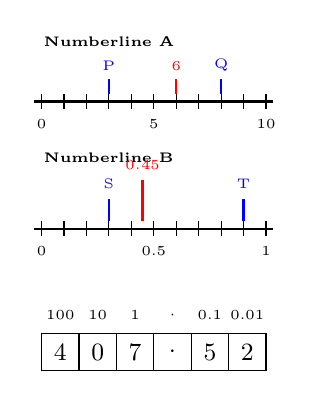
\begin{tikzpicture}[scale=0.95]

% --- Line A: 0 to 10, ticks every 1 ---
\node[font=\tiny\bfseries, anchor=west] at (-0.1,4.6) {Numberline A};
\draw[thick] (-0.1,3.8) -- (3.1,3.8);
\foreach \x in {0,0.3,0.6,0.9,1.2,1.5,1.8,2.1,2.4,2.7,3}
  \draw (\x,3.7) -- (\x,3.9);
\foreach \x/\lab in {0/0,1.5/5,3/10} \node[font=\tiny] at (\x,3.5) {\lab};
% Given points: P at 3, Q at 8. Kept low, so they stay clear of the Line A heading.
\draw[blue, thick] (0.9,3.9) -- (0.9,4.1);
\node[blue, font=\tiny] at (0.9,4.28) {P};
\draw[blue, thick] (2.4,3.9) -- (2.4,4.1);
\node[blue, font=\tiny] at (2.4,4.28) {Q};
% --- Q3 answer: 6 marked on Line A ---
\draw[ans] (1.8,3.9) -- (1.8,4.1);
\node[anslab] at (1.8,4.28) {$6$};

% --- Numberline B: 0 to 1 in tenths ---
\node[font=\tiny\bfseries, anchor=west] at (-0.1,3.05) {Numberline B};
\draw[thick] (-0.1,2.1) -- (3.1,2.1);
\foreach \x in {0,0.3,0.6,0.9,1.2,1.5,1.8,2.1,2.4,2.7,3}
  \draw (\x,2.0) -- (\x,2.2);
\foreach \x/\lab in {0/0,1.5/0.5,3/1} \node[font=\tiny] at (\x,1.8) {\lab};
% Given points: S at 0.3, T at 0.9
\draw[blue, thick] (0.9,2.2) -- (0.9,2.5);
\node[blue, font=\tiny] at (0.9,2.7) {S};
\draw[blue, thick] (2.7,2.2) -- (2.7,2.5);
\node[blue, font=\tiny] at (2.7,2.7) {T};
% --- Q3 answer: 0.45 marked on Line B, raised clear of the blue S label ---
\draw[ans] (1.35,2.2) -- (1.35,2.75);
\node[anslab] at (1.35,2.95) {$0.45$};

% --- Place value chart for 407.52 ---

\foreach \i/\head/\digit in {0/100/4,1/10/0,2/1/7,3/{$\cdot$}/{$\cdot$},4/0.1/5,5/0.01/2} {
  \draw ({0.5*\i},0.2) rectangle ({0.5*\i+0.5},0.7);
  \node[font=\tiny] at ({0.5*\i+0.25},0.95) {\head};
  \node[font=\small] at ({0.5*\i+0.25},0.45) {\digit};
}

\end{tikzpicture}
\end{center}

\column{0.70\textwidth}

\small
\begin{enumerate}\qtight

\ealpara{Na \ealkeytr{osi liczbowej} A jakie liczby są zaznaczone przez $P$ i $Q$?}{On \ealkey{numberline} A what numbers are marked by $P$ and $Q$?}
\item On \ealkey{numberline} A what numbers are marked by $P$ and $Q$? \ashow{\ealpara{$3$ i $8$}{$3$ and $8$}}

\ealpara{Na \ealkeytr{osi liczbowej} B jakie liczby są zaznaczone przez $S$ i $T$?}{On \ealkey{numberline} B what numbers are marked by $S$ and $T$?}
\item On \ealkey{numberline} B what numbers are marked by $S$ and $T$? \ashow{\ealpara{$0.3$ i $0.9$}{$0.3$ and $0.9$}}

\ealpara{Zaznacz $6$ na linii A i $0.45$ na linii B.}{Mark $6$ on Line~A and $0.45$ on Line~B.}
\item Mark $6$ on Line~A and $0.45$ on Line~B.

\end{enumerate}

\end{columns}

\end{frame}

%------------------------------------------------
\begin{frame}{Starter 1 (2 of 3)}

\begin{columns}[T]

\column{0.30\textwidth}
\begin{center}
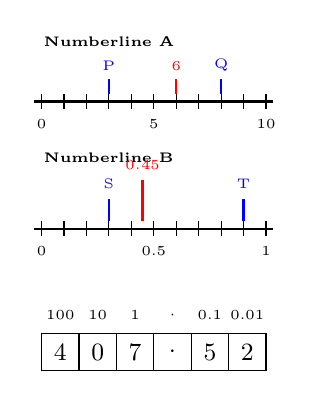
\begin{tikzpicture}[scale=0.95]

% --- Line A: 0 to 10, ticks every 1 ---
\node[font=\tiny\bfseries, anchor=west] at (-0.1,4.6) {Numberline A};
\draw[thick] (-0.1,3.8) -- (3.1,3.8);
\foreach \x in {0,0.3,0.6,0.9,1.2,1.5,1.8,2.1,2.4,2.7,3}
  \draw (\x,3.7) -- (\x,3.9);
\foreach \x/\lab in {0/0,1.5/5,3/10} \node[font=\tiny] at (\x,3.5) {\lab};
% Given points: P at 3, Q at 8. Kept low, so they stay clear of the Line A heading.
\draw[blue, thick] (0.9,3.9) -- (0.9,4.1);
\node[blue, font=\tiny] at (0.9,4.28) {P};
\draw[blue, thick] (2.4,3.9) -- (2.4,4.1);
\node[blue, font=\tiny] at (2.4,4.28) {Q};
% --- Q3 answer: 6 marked on Line A ---
\draw[ans] (1.8,3.9) -- (1.8,4.1);
\node[anslab] at (1.8,4.28) {$6$};

% --- Numberline B: 0 to 1 in tenths ---
\node[font=\tiny\bfseries, anchor=west] at (-0.1,3.05) {Numberline B};
\draw[thick] (-0.1,2.1) -- (3.1,2.1);
\foreach \x in {0,0.3,0.6,0.9,1.2,1.5,1.8,2.1,2.4,2.7,3}
  \draw (\x,2.0) -- (\x,2.2);
\foreach \x/\lab in {0/0,1.5/0.5,3/1} \node[font=\tiny] at (\x,1.8) {\lab};
% Given points: S at 0.3, T at 0.9
\draw[blue, thick] (0.9,2.2) -- (0.9,2.5);
\node[blue, font=\tiny] at (0.9,2.7) {S};
\draw[blue, thick] (2.7,2.2) -- (2.7,2.5);
\node[blue, font=\tiny] at (2.7,2.7) {T};
% --- Q3 answer: 0.45 marked on Line B, raised clear of the blue S label ---
\draw[ans] (1.35,2.2) -- (1.35,2.75);
\node[anslab] at (1.35,2.95) {$0.45$};

% --- Place value chart for 407.52 ---

\foreach \i/\head/\digit in {0/100/4,1/10/0,2/1/7,3/{$\cdot$}/{$\cdot$},4/0.1/5,5/0.01/2} {
  \draw ({0.5*\i},0.2) rectangle ({0.5*\i+0.5},0.7);
  \node[font=\tiny] at ({0.5*\i+0.25},0.95) {\head};
  \node[font=\small] at ({0.5*\i+0.25},0.45) {\digit};
}

\end{tikzpicture}
\end{center}

\column{0.70\textwidth}

\small
\begin{enumerate}\qtight
\setcounter{enumi}{3}

\ealpara{Sam mówi $P=4$, ponieważ to $4$ty znacznik. Co zrobił źle?}{Sam says $P=4$, as it is the $4$th mark. What has he done wrong?}
\item Sam says $P=4$, as it is the $4$th mark. What has he done wrong? \ashow{\ealpara{Policzył znaczniki, a nie \ealkeytr{kroki}: $P=3$}{Counted marks, not \ealkey{steps}: $P=3$}}

\ealpara{Tabela pokazuje $407.52$. Ile jest warte $4$? A ile $5$?}{The chart shows $407.52$. What is the $4$ worth? And the $5$?}
\item The chart shows $407.52$. What is the $4$ worth? And the $5$? \ashow{\ealpara{$400$ i $0.5$}{$400$ and $0.5$}}

\ealpara{Oblicz $407.52\times 10$ i $407.52\div 10$.}{Work out $407.52\times 10$ and $407.52\div 10$.}
\item Work out $407.52\times 10$ and $407.52\div 10$. \ashow{\ealpara{$4075.2$ i $40.752$}{$4075.2$ and $40.752$}}

\end{enumerate}

\end{columns}

\end{frame}

%------------------------------------------------
\begin{frame}{Starter 1 (3 of 3)}

\small
\begin{enumerate}\qtight
\setcounter{enumi}{6}

\ealpara{\ealkeytr{Oś liczbowa} przechodzi od $3.6$ do $3.7$ w $10$ równych \ealkeytr{krokach}. Co znajduje się $3$ \ealkeytr{kroki} od $3.6$?}{A \ealkey{numberline} goes $3.6$ to $3.7$ in $10$ equal \ealkey{steps}. What is $3$ \ealkey{steps} along from $3.6$?}
\item A \ealkey{numberline} goes $3.6$ to $3.7$ in $10$ equal \ealkey{steps}. What is $3$ \ealkey{steps} along from $3.6$? \ashow{\ealpara{$3.63$}{$3.63$}}

\ealpara{Użyj $7$, $5$, $4$, $2$ i \ealkeytr{przecinka dziesiętnego}, aby utworzyć największą liczbę \ealkeytr{mniejszą niż} $100$.}{Use $7$, $5$, $4$, $2$ and a \ealkey{decimal point} to make the largest number \ealkey{less than} $100$.}
\item Use $7$, $5$, $4$, $2$ and a \ealkey{decimal point} to make the largest number \ealkey{less than} $100$. \ashow{\ealpara{$75.42$}{$75.42$}}

\end{enumerate}

\end{frame}

%------------------------------------------------
% STARTER 2: Inequality Symbols and Ordering Decimals
%------------------------------------------------
\begin{frame}{Starter 2: \ealkey{Inequality} Symbols \& \ealkey{Ordering} \ealkey{Decimals} (1 of 3)}

\begin{columns}[T]

\column{0.28\textwidth}
\begin{center}
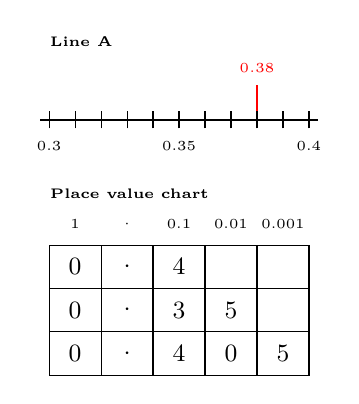
\begin{tikzpicture}[scale=1.1]

% --- Line A: 0.3 to 0.4 in hundredths ---
\node[font=\tiny\bfseries, anchor=west] at (-0.1,3.5) {Line A};
\draw[thick] (-0.1,2.6) -- (3.1,2.6);
\foreach \x in {0,0.3,0.6,0.9,1.2,1.5,1.8,2.1,2.4,2.7,3}
  \draw (\x,2.5) -- (\x,2.7);
\foreach \x/\lab in {0/0.3,1.5/0.35,3/0.4} \node[font=\tiny] at (\x,2.3) {\lab};
% --- Q5 answer: 0.38 marked ---
\draw[ans] (2.4,2.7) -- (2.4,3.0);
\node[anslab] at (2.4,3.2) {$0.38$};

% --- Place value chart: 0.4, 0.35, 0.405 ---
\node[font=\tiny\bfseries, anchor=west] at (-0.1,1.75) {Place value chart};
\foreach \i/\head in {0/1,1/{$\cdot$},2/0.1,3/0.01,4/0.001}
  \node[font=\tiny] at ({0.6*\i+0.3},1.4) {\head};
\foreach \j in {0,1,2} {
  \foreach \i in {0,1,2,3,4}
    \draw ({0.6*\i},{-0.5*\j+1.15}) rectangle ({0.6*\i+0.6},{-0.5*\j+0.65});
}
% row 1: 0.4
\foreach \i/\d in {0/0,1/{$\cdot$},2/4} \node[font=\small] at ({0.6*\i+0.3},0.9) {\d};
% row 2: 0.35
\foreach \i/\d in {0/0,1/{$\cdot$},2/3,3/5} \node[font=\small] at ({0.6*\i+0.3},0.4) {\d};
% row 3: 0.405
\foreach \i/\d in {0/0,1/{$\cdot$},2/4,3/0,4/5} \node[font=\small] at ({0.6*\i+0.3},-0.1) {\d};

\end{tikzpicture}
\end{center}

\column{0.72\textwidth}

\small
\begin{enumerate}\qtight

\ealpara{Wpisz $<$ lub $>$: $7 \mathrel{\text{\ashow{$<$}}} 12$ $30 \mathrel{\text{\ashow{$>$}}} 3$}{Fill in $<$ or $>$: $7 \mathrel{\text{\ashow{$<$}}} 12$ $30 \mathrel{\text{\ashow{$>$}}} 3$}
\item Fill in $<$ or $>$: $7 \mathrel{\text{\ashow{$<$}}} 12$\newline $30 \mathrel{\text{\ashow{$>$}}} 3$

\ealpara{W $0.405$, ile jest warte $4$?}{In $0.405$, what is the $4$ worth?}
\item In $0.405$, what is the $4$ worth? \ashow{\ealpara{$4$ \ealkeytr{części dziesiąte}, $0.4$}{$4$ \ealkey{tenths}, $0.4$}}

\ealpara{Na \ealkeytr{wartości pozycyjnej} tabeli, która jest większa, $0.4$ czy $0.35$? Dlaczego?}{On the \ealkey{place value} chart, which is bigger, $0.4$ or $0.35$? Why?}
\item On the \ealkey{place value} chart, which is bigger, $0.4$ or $0.35$? Why? \ashow{\ealpara{$0.4$: $4$ \ealkeytr{części dziesiąte} są \ealkeytr{większe niż} $3$ \ealkeytr{części dziesiąte}}{$0.4$: $4$ \ealkey{tenths} is \ealkey{greater than} $3$ \ealkey{tenths}}}

\end{enumerate}

\end{columns}

\end{frame}

%------------------------------------------------
\begin{frame}{Starter 2: \ealkey{Inequality} Symbols \& \ealkey{Ordering} \ealkey{Decimals} (2 of 3)}

\begin{columns}[T]

\column{0.28\textwidth}
\begin{center}
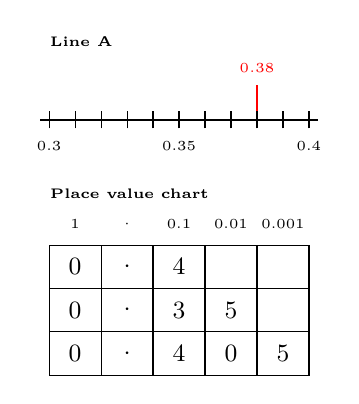
\begin{tikzpicture}[scale=1.1]

% --- Line A: 0.3 to 0.4 in hundredths ---
\node[font=\tiny\bfseries, anchor=west] at (-0.1,3.5) {Line A};
\draw[thick] (-0.1,2.6) -- (3.1,2.6);
\foreach \x in {0,0.3,0.6,0.9,1.2,1.5,1.8,2.1,2.4,2.7,3}
  \draw (\x,2.5) -- (\x,2.7);
\foreach \x/\lab in {0/0.3,1.5/0.35,3/0.4} \node[font=\tiny] at (\x,2.3) {\lab};
% --- Q5 answer: 0.38 marked ---
\draw[ans] (2.4,2.7) -- (2.4,3.0);
\node[anslab] at (2.4,3.2) {$0.38$};

% --- Place value chart: 0.4, 0.35, 0.405 ---
\node[font=\tiny\bfseries, anchor=west] at (-0.1,1.75) {Place value chart};
\foreach \i/\head in {0/1,1/{$\cdot$},2/0.1,3/0.01,4/0.001}
  \node[font=\tiny] at ({0.6*\i+0.3},1.4) {\head};
\foreach \j in {0,1,2} {
  \foreach \i in {0,1,2,3,4}
    \draw ({0.6*\i},{-0.5*\j+1.15}) rectangle ({0.6*\i+0.6},{-0.5*\j+0.65});
}
% row 1: 0.4
\foreach \i/\d in {0/0,1/{$\cdot$},2/4} \node[font=\small] at ({0.6*\i+0.3},0.9) {\d};
% row 2: 0.35
\foreach \i/\d in {0/0,1/{$\cdot$},2/3,3/5} \node[font=\small] at ({0.6*\i+0.3},0.4) {\d};
% row 3: 0.405
\foreach \i/\d in {0/0,1/{$\cdot$},2/4,3/0,4/5} \node[font=\small] at ({0.6*\i+0.3},-0.1) {\d};

\end{tikzpicture}
\end{center}

\column{0.72\textwidth}

\small
\begin{enumerate}\qtight
\setcounter{enumi}{3}

\ealpara{Wpisz $<$, $>$ lub $=$ $0.4 \mathrel{\text{\ashow{$=$}}} 0.40$, $0.6 \mathrel{\text{\ashow{$>$}}} 0.06$}{Fill in $<$, $>$ or $=$ $0.4 \mathrel{\text{\ashow{$=$}}} 0.40$, $0.6 \mathrel{\text{\ashow{$>$}}} 0.06$}
\item Fill in $<$, $>$ or $=$ $0.4 \mathrel{\text{\ashow{$=$}}} 0.40$, $0.6 \mathrel{\text{\ashow{$>$}}} 0.06$

\ealpara{Zaznacz $0.38$ na linii A. Czy jest bliżej $0.3$ czy $0.4$?}{Mark $0.38$ on Line A. Is it nearer $0.3$ or $0.4$?}
\item Mark $0.38$ on Line A. Is it nearer $0.3$ or $0.4$? \ashow{\ealpara{bliżej $0.4$}{nearer $0.4$}}

\ealpara{\ealkeytr{Uporządkuj} od najmniejszej do największej: $0.5$, $0.45$, $0.405$, $0.54$}{\ealkey{Order}, smallest first: $0.5$, $0.45$, $0.405$, $0.54$}
\item \ealkey{Order}, smallest first: $0.5$, $0.45$, $0.405$, $0.54$ \ashow{$0.405$, $0.45$, $0.5$, $0.54$}

\end{enumerate}

\end{columns}

\end{frame}

%------------------------------------------------
\begin{frame}{Starter 2: \ealkey{Inequality} Symbols \& \ealkey{Ordering} \ealkey{Decimals} (3 of 3)}

\small
\begin{enumerate}\qtight
\setcounter{enumi}{6}

\ealpara{Prawda czy fałsz: więcej \ealkeytr{cyfr} \emph{po} \ealkeytr{przecinku dziesiętnym} oznacza większą liczbę? Podaj przykład/kontrprzykład.}{True or false: more \ealkey{digits} \emph{after} the \ealkey{decimal point} means a bigger number? Give an example/counter-example.}
\item True or false: more \ealkey{digits} \emph{after} the \ealkey{decimal point} means a bigger number? Give an example/counter-example. \ashow{\ealpara{Fałsz: $0.9>0.1234$}{False: $0.9>0.1234$}}

\ealpara{Alfie mówi $0.45>0.5$, ponieważ $45>5$. Wyjaśnij jego błąd, a następnie zapisz \ealkeytr{ułamek dziesiętny} między $0.4$ a $0.405$.}{Alfie says $0.45>0.5$ as $45>5$. Explain his mistake, then write a \ealkey{decimal} between $0.4$ and $0.405$.}
\item Alfie says $0.45>0.5$ as $45>5$. Explain his mistake, then write a \ealkey{decimal} between $0.4$ and $0.405$. \ashow{\ealpara{$0.5$ ma $5$ \ealkeytr{części dziesiąte}; np.\ $0.402$}{$0.5$ has $5$ \ealkey{tenths}; e.g.\ $0.402$}}

\end{enumerate}

\end{frame}

%------------------------------------------------
% STARTER 3: Negative Numbers
%------------------------------------------------
\begin{frame}{Starter 3: \ealkey{Ordering} \ealkey{Negative Numbers} (1 of 3)}

\begin{columns}[T]

\column{0.30\textwidth}
\begin{center}
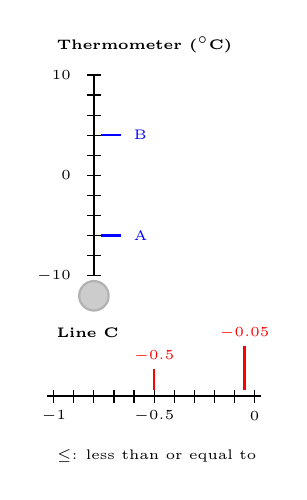
\begin{tikzpicture}[scale=0.85]

% --- Thermometer: -10 to 10, one tick every 2 degrees, only -10/0/10 labelled ---
\node[font=\tiny\bfseries, anchor=west] at (-0.1,3.45) {Thermometer ($^\circ$C)};
\draw[thick] (0.6,0) -- (0.6,3);
\foreach \y in {0,0.3,0.6,0.9,1.2,1.5,1.8,2.1,2.4,2.7,3}
  \draw (0.5,\y) -- (0.7,\y);
\foreach \y/\lab in {0/{$-10$},1.5/{$0$},3/{$10$}}
  \node[font=\tiny, anchor=east] at (0.4,\y) {\lab};
\fill[gray!40] (0.6,-0.3) circle (0.22);
\draw[gray!60, thick] (0.6,-0.3) circle (0.22);
% Given readings: A at -6, B at 4 (both sit exactly on a tick)
\draw[blue, thick] (0.7,0.6) -- (1.0,0.6);
\node[blue, font=\tiny, anchor=west] at (1.05,0.6) {A};
\draw[blue, thick] (0.7,2.1) -- (1.0,2.1);
\node[blue, font=\tiny, anchor=west] at (1.05,2.1) {B};

% --- Line C: -1 to 0 in tenths ---
\node[font=\tiny\bfseries, anchor=west] at (-0.1,-0.85) {Line C};
\draw[thick] (-0.1,-1.8) -- (3.1,-1.8);
\foreach \x in {0,0.3,0.6,0.9,1.2,1.5,1.8,2.1,2.4,2.7,3}
  \draw (\x,-1.9) -- (\x,-1.7);
\foreach \x/\lab in {0/{$-1$},1.5/{$-0.5$},3/{$0$}} \node[font=\tiny] at (\x,-2.1) {\lab};
% Reminder for the challenge question, which is the deck's only use of a weak inequality
\node[font=\tiny, anchor=west] at (-0.1,-2.7) {$\leq$: less than or equal to};
% --- Q5 answers: -0.5 and -0.05 marked on Line C, at different heights ---
\draw[ans] (1.5,-1.7) -- (1.5,-1.4);
\node[anslab] at (1.5,-1.2) {$-0.5$};
\draw[ans] (2.85,-1.7) -- (2.85,-1.05);
\node[anslab] at (2.85,-0.85) {$-0.05$};

\end{tikzpicture}
\end{center}

\column{0.70\textwidth}

\small
\begin{enumerate}\qtight

\ealpara{Która jest zimniejsza, $4\,^\circ$C czy $-4\,^\circ$C?}{Which is colder, $4\,^\circ$C or $-4\,^\circ$C?}
\item Which is colder, $4\,^\circ$C or $-4\,^\circ$C? \ashow{\ealpara{$-4\,^\circ$C}{$-4\,^\circ$C}}

\ealpara{Ile jest wart każdy znacznik na termometrze? Zapisz temperatury w A i B.}{What is each mark on the thermometer worth? Write the temperatures at A and B.}
\item What is each mark on the thermometer worth? Write the temperatures at A and B. \ashow{\ealpara{$2\,^\circ$C na znacznik; A $=-6$, B $=4$}{$2\,^\circ$C per mark; A $=-6$, B $=4$}}

\ealpara{Która jest zimniejsza, $-3$ czy $-8$? Wpisz: $-3 \mathrel{\text{\ashowq{$>$}}} -8$}{Which is colder, $-3$ or $-8$? Fill in: $-3 \mathrel{\text{\ashowq{$>$}}} -8$}
\item Which is colder, $-3$ or $-8$? Fill in: $-3 \mathrel{\text{\ashowq{$>$}}} -8$ \ashow{\ealpara{($-8$ jest zimniejsza)}{($-8$ is colder)}}

\end{enumerate}

\end{columns}

\end{frame}

%------------------------------------------------
\begin{frame}{Starter 3: \ealkey{Ordering} \ealkey{Negative Numbers} (2 of 3)}

\begin{columns}[T]

\column{0.30\textwidth}
\begin{center}
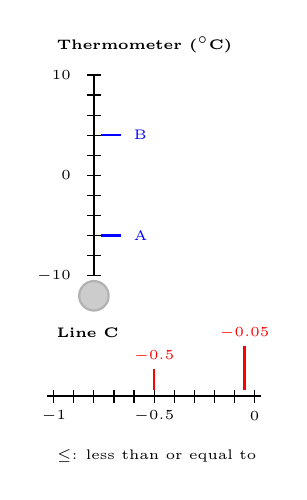
\begin{tikzpicture}[scale=0.85]

% --- Thermometer: -10 to 10, one tick every 2 degrees, only -10/0/10 labelled ---
\node[font=\tiny\bfseries, anchor=west] at (-0.1,3.45) {Thermometer ($^\circ$C)};
\draw[thick] (0.6,0) -- (0.6,3);
\foreach \y in {0,0.3,0.6,0.9,1.2,1.5,1.8,2.1,2.4,2.7,3}
  \draw (0.5,\y) -- (0.7,\y);
\foreach \y/\lab in {0/{$-10$},1.5/{$0$},3/{$10$}}
  \node[font=\tiny, anchor=east] at (0.4,\y) {\lab};
\fill[gray!40] (0.6,-0.3) circle (0.22);
\draw[gray!60, thick] (0.6,-0.3) circle (0.22);
% Given readings: A at -6, B at 4 (both sit exactly on a tick)
\draw[blue, thick] (0.7,0.6) -- (1.0,0.6);
\node[blue, font=\tiny, anchor=west] at (1.05,0.6) {A};
\draw[blue, thick] (0.7,2.1) -- (1.0,2.1);
\node[blue, font=\tiny, anchor=west] at (1.05,2.1) {B};

% --- Line C: -1 to 0 in tenths ---
\node[font=\tiny\bfseries, anchor=west] at (-0.1,-0.85) {Line C};
\draw[thick] (-0.1,-1.8) -- (3.1,-1.8);
\foreach \x in {0,0.3,0.6,0.9,1.2,1.5,1.8,2.1,2.4,2.7,3}
  \draw (\x,-1.9) -- (\x,-1.7);
\foreach \x/\lab in {0/{$-1$},1.5/{$-0.5$},3/{$0$}} \node[font=\tiny] at (\x,-2.1) {\lab};
% Reminder for the challenge question, which is the deck's only use of a weak inequality
\node[font=\tiny, anchor=west] at (-0.1,-2.7) {$\leq$: less than or equal to};
% --- Q5 answers: -0.5 and -0.05 marked on Line C, at different heights ---
\draw[ans] (1.5,-1.7) -- (1.5,-1.4);
\node[anslab] at (1.5,-1.2) {$-0.5$};
\draw[ans] (2.85,-1.7) -- (2.85,-1.05);
\node[anslab] at (2.85,-0.85) {$-0.05$};

\end{tikzpicture}
\end{center}

\column{0.70\textwidth}

\small
\begin{enumerate}\qtight
\setcounter{enumi}{3}

\ealpara{\ealkeytr{Uporządkuj} od najmniejszej do największej: $-2$, $5$, $-7$, $0$, $-1$}{\ealkey{Order}, smallest first: $-2$, $5$, $-7$, $0$, $-1$}
\item \ealkey{Order}, smallest first: $-2$, $5$, $-7$, $0$, $-1$ \ashow{\ealpara{($-7,-2,-1,0,5$)}{($-7,-2,-1,0,5$)}}

\ealpara{Zaznacz $-0.5$ i $-0.05$ na linii C. Która jest większa?}{Mark $-0.5$ and $-0.05$ on Line C. Which is larger?}
\item Mark $-0.5$ and $-0.05$ on Line C. Which is larger? \ashow{\ealpara{$-0.05$}{$-0.05$}}

\ealpara{Wpisz $<$ lub $>$: $-4.5 \mathrel{\text{\ashowq{$<$}}} -4.05$, $-0.3 \mathrel{\text{\ashowq{$<$}}} 0.03$}{Fill in $<$ or $>$: $-4.5 \mathrel{\text{\ashowq{$<$}}} -4.05$, $-0.3 \mathrel{\text{\ashowq{$<$}}} 0.03$}
\item Fill in $<$ or $>$: $-4.5 \mathrel{\text{\ashowq{$<$}}} -4.05$, $-0.3 \mathrel{\text{\ashowq{$<$}}} 0.03$

\end{enumerate}

\end{columns}

\end{frame}

%------------------------------------------------
\begin{frame}{Starter 3: \ealkey{Ordering} \ealkey{Negative Numbers} (3 of 3)}

\begin{columns}[T]

\column{0.30\textwidth}
\begin{center}
\ealpara{$\leq$: \ealkeytr{mniejsze lub równe}}{$\leq$: \ealkey{less than or equal to}}
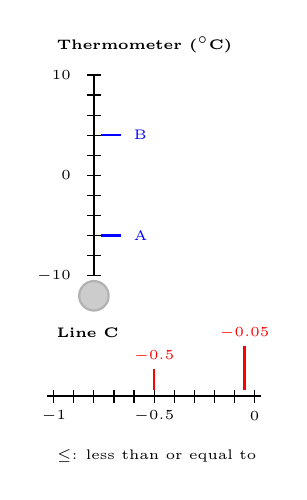
\begin{tikzpicture}[scale=0.85]

% --- Thermometer: -10 to 10, one tick every 2 degrees, only -10/0/10 labelled ---
\node[font=\tiny\bfseries, anchor=west] at (-0.1,3.45) {Thermometer ($^\circ$C)};
\draw[thick] (0.6,0) -- (0.6,3);
\foreach \y in {0,0.3,0.6,0.9,1.2,1.5,1.8,2.1,2.4,2.7,3}
  \draw (0.5,\y) -- (0.7,\y);
\foreach \y/\lab in {0/{$-10$},1.5/{$0$},3/{$10$}}
  \node[font=\tiny, anchor=east] at (0.4,\y) {\lab};
\fill[gray!40] (0.6,-0.3) circle (0.22);
\draw[gray!60, thick] (0.6,-0.3) circle (0.22);
% Given readings: A at -6, B at 4 (both sit exactly on a tick)
\draw[blue, thick] (0.7,0.6) -- (1.0,0.6);
\node[blue, font=\tiny, anchor=west] at (1.05,0.6) {A};
\draw[blue, thick] (0.7,2.1) -- (1.0,2.1);
\node[blue, font=\tiny, anchor=west] at (1.05,2.1) {B};

% --- Line C: -1 to 0 in tenths ---
\node[font=\tiny\bfseries, anchor=west] at (-0.1,-0.85) {Line C};
\draw[thick] (-0.1,-1.8) -- (3.1,-1.8);
\foreach \x in {0,0.3,0.6,0.9,1.2,1.5,1.8,2.1,2.4,2.7,3}
  \draw (\x,-1.9) -- (\x,-1.7);
\foreach \x/\lab in {0/{$-1$},1.5/{$-0.5$},3/{$0$}} \node[font=\tiny] at (\x,-2.1) {\lab};
% Reminder for the challenge question, which is the deck's only use of a weak inequality
\node[font=\tiny, anchor=west] at (-0.1,-2.7) {$\leq$: less than or equal to};
% --- Q5 answers: -0.5 and -0.05 marked on Line C, at different heights ---
\draw[ans] (1.5,-1.7) -- (1.5,-1.4);
\node[anslab] at (1.5,-1.2) {$-0.5$};
\draw[ans] (2.85,-1.7) -- (2.85,-1.05);
\node[anslab] at (2.85,-0.85) {$-0.05$};

\end{tikzpicture}
\end{center}

\column{0.70\textwidth}

\small
\begin{enumerate}\qtight
\setcounter{enumi}{6}

\ealpara{(Rozszerzenie) \ealkeytr{Uporządkuj} od najmniejszej do największej: $-0.08$, $0.7$, $-0.8$, $-0.75$}{(Extension) \ealkey{Order}, smallest first: $-0.08$, $0.7$, $-0.8$, $-0.75$}
\item (Extension) \ealkey{Order}, smallest first: $-0.08$, $0.7$, $-0.8$, $-0.75$ \ashow{\ealpara{($-0.8$, $-0.75$, $-0.08$, $0.7$)}{($-0.8$, $-0.75$, $-0.08$, $0.7$)}}

\ealpara{(Wyzwanie) Wypisz \ealkeytr{liczby całkowite} $n$: $-3\leq n<2$. Zapisz liczbę między $-0.5$ a $-0.4$.}{(Challenge) List the \ealkey{integers} $n$: $-3\leq n<2$. Write a number between $-0.5$ and $-0.4$.}
\item (Challenge) List the \ealkey{integers} $n$: $-3\leq n<2$. Write a number between $-0.5$ and $-0.4$. \ashow{\ealpara{$-3,-2,-1,0,1$; np.\ $-0.45$}{$-3,-2,-1,0,1$; e.g.\ $-0.45$}}

\end{enumerate}

\end{columns}

\end{frame}

%------------------------------------------------
% STARTER 4: Rounding Integers
%------------------------------------------------
\begin{frame}{Starter 4: \ealkey{Rounding} \ealkey{Integers} (1 of 3)}

\begin{columns}[T]

\column{0.30\textwidth}
\begin{center}
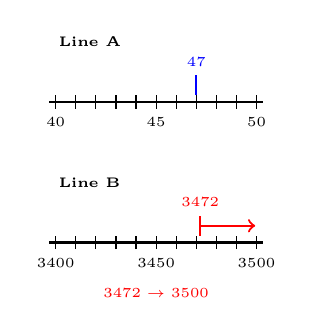
\begin{tikzpicture}[scale=0.85]

% --- Line A: 40 to 50, ticks every 1 ---
\node[font=\tiny\bfseries, anchor=west] at (-0.1,3.5) {Line A};
\draw[thick] (-0.1,2.6) -- (3.1,2.6);
\foreach \x in {0,0.3,0.6,0.9,1.2,1.5,1.8,2.1,2.4,2.7,3}
  \draw (\x,2.5) -- (\x,2.7);
\foreach \x/\lab in {0/40,1.5/45,3/50} \node[font=\tiny] at (\x,2.3) {\lab};
% Given point: 47
\draw[blue, thick] (2.1,2.7) -- (2.1,3.0);
\node[blue, font=\tiny] at (2.1,3.2) {$47$};

% --- Line B: 3400 to 3500, ticks every 10 ---
\node[font=\tiny\bfseries, anchor=west] at (-0.1,1.4) {Line B};
\draw[thick] (-0.1,0.5) -- (3.1,0.5);
\foreach \x in {0,0.3,0.6,0.9,1.2,1.5,1.8,2.1,2.4,2.7,3}
  \draw (\x,0.4) -- (\x,0.6);
\foreach \x/\lab in {0/3400,1.5/3450,3/3500} \node[font=\tiny] at (\x,0.2) {\lab};
% --- Q4 answers: 3472 marked, with an arrow to the nearer end ---
\draw[ans] (2.16,0.6) -- (2.16,0.9);
\node[anslab] at (2.16,1.1) {$3472$};
\draw[ans, ->] (2.16,0.75) -- (2.98,0.75);
\node[anslab] at (1.5,-0.25) {$3472 \to 3500$};

\end{tikzpicture}
\end{center}

\column{0.70\textwidth}

\small
\begin{enumerate}\qtight

\ealpara{Wpisz $<$ lub $>$: $-6 \mathrel{\text{\ashowq{$<$}}} -2$}{Fill in $<$ or $>$: $-6 \mathrel{\text{\ashowq{$<$}}} -2$}
\item Fill in $<$ or $>$: $-6 \mathrel{\text{\ashowq{$<$}}} -2$

\ealpara{Linia A: czy $47$ jest bliżej $40$ czy $50$? \ealkeytr{Zaokrąglij} do najbliższych $10$.}{Line A: is $47$ nearer $40$ or $50$? \ealkey{Round} it to the nearest $10$.}
\item Line A: is $47$ nearer $40$ or $50$? \ealkey{Round} it to the nearest $10$. \ashow{\ealpara{bliżej $50$, więc $50$}{nearer $50$, so $50$}}

\ealpara{\ealkeytr{Zaokrąglij} do najbliższych $10$: $32$, $85$}{\ealkey{Round} to the nearest $10$: $32$, $85$}
\item \ealkey{Round} to the nearest $10$: $32$, $85$ \ashow{\ealpara{($30$ i $90$)}{($30$ and $90$)}}

\end{enumerate}

\end{columns}

\end{frame}

%------------------------------------------------
\begin{frame}{Starter 4: \ealkey{Rounding} \ealkey{Integers} (2 of 3)}

\begin{columns}[T]

\column{0.30\textwidth}
\begin{center}
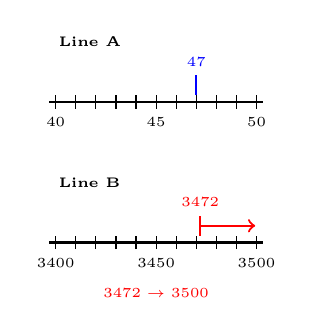
\begin{tikzpicture}[scale=0.85]

% --- Line A: 40 to 50, ticks every 1 ---
\node[font=\tiny\bfseries, anchor=west] at (-0.1,3.5) {Line A};
\draw[thick] (-0.1,2.6) -- (3.1,2.6);
\foreach \x in {0,0.3,0.6,0.9,1.2,1.5,1.8,2.1,2.4,2.7,3}
  \draw (\x,2.5) -- (\x,2.7);
\foreach \x/\lab in {0/40,1.5/45,3/50} \node[font=\tiny] at (\x,2.3) {\lab};
% Given point: 47
\draw[blue, thick] (2.1,2.7) -- (2.1,3.0);
\node[blue, font=\tiny] at (2.1,3.2) {$47$};

% --- Line B: 3400 to 3500, ticks every 10 ---
\node[font=\tiny\bfseries, anchor=west] at (-0.1,1.4) {Line B};
\draw[thick] (-0.1,0.5) -- (3.1,0.5);
\foreach \x in {0,0.3,0.6,0.9,1.2,1.5,1.8,2.1,2.4,2.7,3}
  \draw (\x,0.4) -- (\x,0.6);
\foreach \x/\lab in {0/3400,1.5/3450,3/3500} \node[font=\tiny] at (\x,0.2) {\lab};
% --- Q4 answers: 3472 marked, with an arrow to the nearer end ---
\draw[ans] (2.16,0.6) -- (2.16,0.9);
\node[anslab] at (2.16,1.1) {$3472$};
\draw[ans, ->] (2.16,0.75) -- (2.98,0.75);
\node[anslab] at (1.5,-0.25) {$3472 \to 3500$};

\end{tikzpicture}
\end{center}

\column{0.70\textwidth}

\small
\begin{enumerate}\qtight
\setcounter{enumi}{3}

\ealpara{Zaznacz $3472$ na linii B, a następnie \ealkeytr{zaokrąglij} do najbliższych $100$.}{Mark $3472$ on Line B, then \ealkey{round} it to the nearest $100$.}
\item Mark $3472$ on Line B, then \ealkey{round} it to the nearest $100$.

\ealpara{\ealkeytr{Zaokrąglij} $3472$ do najbliższych $10$; do najbliższych $1000$.}{\ealkey{Round} $3472$ to the nearest $10$; to the nearest $1000$.}
\item \ealkey{Round} $3472$ to the nearest $10$; to the nearest $1000$. \ashow{\ealpara{$3470$ i $3000$}{$3470$ and $3000$}}

\ealpara{\ealkeytr{Zaokrąglij} $4950$ do najbliższych $100$.}{\ealkey{Round} $4950$ to the nearest $100$.}
\item \ealkey{Round} $4950$ to the nearest $100$. \ashow{\ealpara{$5000$}{$5000$}}

\end{enumerate}

\end{columns}

\end{frame}

%------------------------------------------------
\begin{frame}{Starter 4: \ealkey{Rounding} \ealkey{Integers} (3 of 3)}

\small
\begin{enumerate}\qtight
\setcounter{enumi}{6}

\ealpara{Zoe \ealkeytr{zaokrągla} $8449$ do najbliższych $100$: $8449\to 8450\to 8500$. Jaki jest jej błąd?}{Zoe \ealkey{rounds} $8449$ to the nearest $100$: $8449\to 8450\to 8500$. What is her mistake?}
\item Zoe \ealkey{rounds} $8449$ to the nearest $100$: $8449\to 8450\to 8500$. What is her mistake? \ashow{\ealpara{\ealkeytr{Zaokrągliła} dwa razy: tylko \ealkeytr{cyfra dziesiątek} $4$ się liczy, więc $8400$}{\ealkey{Rounded} twice: only the \ealkey{tens digit} $4$ counts, so $8400$}}

\ealpara{Liczba \ealkeytr{zaokrąglona} do najbliższych $10$ to $250$. Jaka może być najmniejsza? Największa?}{A number \ealkey{rounded} to the nearest $10$ is $250$. What is the smallest it could be? The largest?}
\item A number \ealkey{rounded} to the nearest $10$ is $250$. What is the smallest it could be? The largest? \ashow{\ealpara{$245$ i $254$}{$245$ and $254$}}

\end{enumerate}

\end{frame}

%------------------------------------------------
% STARTER 5: Rounding Decimals, Recurring and Irrational
%------------------------------------------------
\begin{frame}{Starter 5: \ealkey{Rounding} \ealkey{Decimals} \& Never-Ending \ealkey{Decimals} (1 of 3)}

\begin{columns}[T]

\column{0.30\textwidth}
\begin{center}
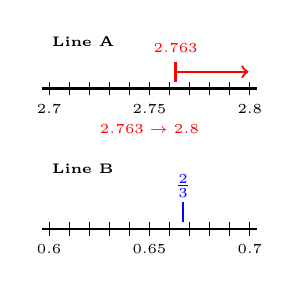
\begin{tikzpicture}[scale=0.85]

% --- Line A: 2.7 to 2.8 in hundredths ---
\node[font=\tiny\bfseries, anchor=west] at (-0.1,3.3) {Line A};
\draw[thick] (-0.1,2.6) -- (3.1,2.6);
\foreach \x in {0,0.3,0.6,0.9,1.2,1.5,1.8,2.1,2.4,2.7,3}
  \draw (\x,2.5) -- (\x,2.7);
\foreach \x/\lab in {0/2.7,1.5/2.75,3/2.8} \node[font=\tiny] at (\x,2.3) {\lab};
% --- Q3 answers: 2.763 marked, with an arrow to the nearer end ---
\draw[ans] (1.89,2.7) -- (1.89,3.0);
\node[anslab] at (1.89,3.2) {$2.763$};
\draw[ans, ->] (1.89,2.85) -- (2.98,2.85);
\node[anslab] at (1.5,2.0) {$2.763 \to 2.8$};

% --- Line B: 0.6 to 0.7 in hundredths, with 2/3 shown ---
\node[font=\tiny\bfseries, anchor=west] at (-0.1,1.4) {Line B};
\draw[thick] (-0.1,0.5) -- (3.1,0.5);
\foreach \x in {0,0.3,0.6,0.9,1.2,1.5,1.8,2.1,2.4,2.7,3}
  \draw (\x,0.4) -- (\x,0.6);
\foreach \x/\lab in {0/0.6,1.5/0.65,3/0.7} \node[font=\tiny] at (\x,0.2) {\lab};
% Given point: 2/3 = 0.6666...
\draw[blue, thick] (2.0,0.6) -- (2.0,0.9);
\node[blue, font=\scriptsize] at (2.0,1.15) {$\tfrac{2}{3}$};

\end{tikzpicture}

\vspace{0.4em}
{\scriptsize
\begin{tabular}{@{}l@{}}
\textbf{Never-ending decimals} \\[0.15em]
$\frac{2}{3} = 0.6666\ldots = 0.\dot{6}$ \\
$\frac{1}{7} = 0.142857142857\ldots$ \\
$\pi = 3.14159265\ldots$ \\
$\sqrt{2} = 1.41421356\ldots$ \\
$0.1010010001\ldots$
\end{tabular}}
\end{center}

\column{0.70\textwidth}

\small
\begin{enumerate}\qtight

\ealpara{\ealkeytr{Zaokrąglij} $4738$ do najbliższych $100$.}{\ealkey{Round} $4738$ to the nearest $100$.}
\item \ealkey{Round} $4738$ to the nearest $100$. \ashow{\ealpara{$4700$}{$4700$}}

\ealpara{\ealkeytr{Zaokrąglij} do najbliższej \ealkeytr{liczby całkowitej nieujemnej}: $4.6$, $12.348$}{\ealkey{Round} to the nearest \ealkey{whole number}: $4.6$, $12.348$}
\item \ealkey{Round} to the nearest \ealkey{whole number}: $4.6$, $12.348$ \ashow{\ealpara{($5$ i $12$)}{($5$ and $12$)}}

\ealpara{Zaznacz $2.763$ na linii A. \ealkeytr{Zaokrąglij} do $1$ \ealkeytr{miejsca dziesiętnego} (m.d.).}{Mark $2.763$ on Line A. \ealkey{Round} it to $1$ \ealkey{decimal place} (d.p.).}
\item Mark $2.763$ on Line A. \ealkey{Round} it to $1$ \ealkey{decimal place} (d.p.).

\end{enumerate}

\end{columns}

\end{frame}

%------------------------------------------------
\begin{frame}{Starter 5: \ealkey{Rounding} \ealkey{Decimals} \& Never-Ending \ealkey{Decimals} (2 of 3)}

\begin{columns}[T]

\column{0.30\textwidth}
\begin{center}
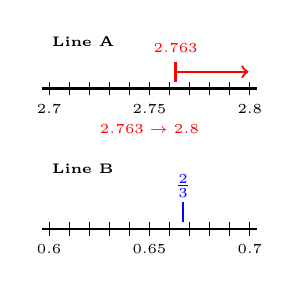
\begin{tikzpicture}[scale=0.85]

% --- Line A: 2.7 to 2.8 in hundredths ---
\node[font=\tiny\bfseries, anchor=west] at (-0.1,3.3) {Line A};
\draw[thick] (-0.1,2.6) -- (3.1,2.6);
\foreach \x in {0,0.3,0.6,0.9,1.2,1.5,1.8,2.1,2.4,2.7,3}
  \draw (\x,2.5) -- (\x,2.7);
\foreach \x/\lab in {0/2.7,1.5/2.75,3/2.8} \node[font=\tiny] at (\x,2.3) {\lab};
% --- Q3 answers: 2.763 marked, with an arrow to the nearer end ---
\draw[ans] (1.89,2.7) -- (1.89,3.0);
\node[anslab] at (1.89,3.2) {$2.763$};
\draw[ans, ->] (1.89,2.85) -- (2.98,2.85);
\node[anslab] at (1.5,2.0) {$2.763 \to 2.8$};

% --- Line B: 0.6 to 0.7 in hundredths, with 2/3 shown ---
\node[font=\tiny\bfseries, anchor=west] at (-0.1,1.4) {Line B};
\draw[thick] (-0.1,0.5) -- (3.1,0.5);
\foreach \x in {0,0.3,0.6,0.9,1.2,1.5,1.8,2.1,2.4,2.7,3}
  \draw (\x,0.4) -- (\x,0.6);
\foreach \x/\lab in {0/0.6,1.5/0.65,3/0.7} \node[font=\tiny] at (\x,0.2) {\lab};
% Given point: 2/3 = 0.6666...
\draw[blue, thick] (2.0,0.6) -- (2.0,0.9);
\node[blue, font=\scriptsize] at (2.0,1.15) {$\tfrac{2}{3}$};

\end{tikzpicture}

\vspace{0.4em}
{\scriptsize
\begin{tabular}{@{}l@{}}
\textbf{Never-ending decimals} \\[0.15em]
$\frac{2}{3} = 0.6666\ldots = 0.\dot{6}$ \\
$\frac{1}{7} = 0.142857142857\ldots$ \\
$\pi = 3.14159265\ldots$ \\
$\sqrt{2} = 1.41421356\ldots$ \\
$0.1010010001\ldots$
\end{tabular}}
\end{center}

\column{0.70\textwidth}

\small
\begin{enumerate}\qtight
\setcounter{enumi}{3}

\ealpara{\ealkeytr{Zaokrąglij} do $1$ m.d.: $4.62$, $0.95$. Dlaczego $0.95$ to nie $1$?}{\ealkey{Round} to $1$ d.p.: $4.62$, $0.95$. Why is $0.95$ not $1$?}
\item \ealkey{Round} to $1$ d.p.: $4.62$, $0.95$. Why is $0.95$ not $1$? \ashow{\ealpara{$4.6$, $1.0$ --- $1$ m.d.\ potrzebuje jednej \ealkeytr{cyfry} dziesiętnej}{$4.6$, $1.0$ --- $1$ d.p.\ needs one decimal \ealkey{digit}}}

\ealpara{\ealkeytr{Zaokrąglij} $12.348$ do $2$ m.d., następnie do $1$ m.d. Dlaczego nie $12.4$?}{\ealkey{Round} $12.348$ to $2$ d.p., then to $1$ d.p. Why not $12.4$?}
\item \ealkey{Round} $12.348$ to $2$ d.p., then to $1$ d.p. Why not $12.4$? \ashow{\ealpara{$12.35$, $12.3$ --- nigdy nie \ealkeytr{zaokrąglaj} dwa razy}{$12.35$, $12.3$ --- never \ealkey{round} twice}}

\ealpara{Linia B pokazuje $\frac{2}{3}=0.\dot{6}$. \ealkeytr{Zaokrąglij} do $1$ m.d.\ i $2$ m.d.}{Line B shows $\frac{2}{3}=0.\dot{6}$. \ealkey{Round} it to $1$ d.p.\ and $2$ d.p.}
\item Line B shows $\frac{2}{3}=0.\dot{6}$. \ealkey{Round} it to $1$ d.p.\ and $2$ d.p. \ashow{\ealpara{$0.7$ i $0.67$}{$0.7$ and $0.67$}}

\end{enumerate}

\end{columns}

\end{frame}

%------------------------------------------------
\begin{frame}{Starter 5: \ealkey{Rounding} \ealkey{Decimals} \& Never-Ending \ealkey{Decimals} (3 of 3)}

\begin{center}
{\scriptsize
\begin{tabular}{@{}l@{}}
\textbf{Never-ending decimals} \\[0.15em]
$\frac{2}{3} = 0.6666\ldots = 0.\dot{6}$ \\
$\frac{1}{7} = 0.142857142857\ldots$ \\
$\pi = 3.14159265\ldots$ \\
$\sqrt{2} = 1.41421356\ldots$ \\
$0.1010010001\ldots$
\end{tabular}}
\end{center}

\vspace{0.5em}

\small
\begin{enumerate}\qtight
\setcounter{enumi}{6}

\ealpara{(Rozszerzenie) Zapisz $\frac{1}{3}$ w \ealkeytr{notacji kropkowej}, następnie \ealkeytr{zaokrąglij} $\frac{1}{7}$ do $3$ m.d.}{(Extension) Write $\frac{1}{3}$ in \ealkey{dot notation}, then \ealkey{round} $\frac{1}{7}$ to $3$ d.p.}
\item (Extension) Write $\frac{1}{3}$ in \ealkey{dot notation}, then \ealkey{round} $\frac{1}{7}$ to $3$ d.p. \ashow{\ealpara{$0.\dot{3}$ i $0.143$}{$0.\dot{3}$ and $0.143$}}

\ealpara{(Wyzwanie) Które wymienione \ealkeytr{ułamki dziesiętne} nigdy nie tworzą \ealkeytr{okresu}? Czy któryś może nadal być \ealkeytr{ułamkiem}?}{(Challenge) Which listed \ealkey{decimals} never settle into a \ealkey{repeating block}? Can one still be a \ealkey{fraction}?}
\item (Challenge) Which listed \ealkey{decimals} never settle into a \ealkey{repeating block}? Can one still be a \ealkey{fraction}? \ashow{\ealpara{$\pi$, $\sqrt{2}$, $0.101001\ldots$; tak: $0.\dot{3}=\frac13$}{$\pi$, $\sqrt{2}$, $0.101001\ldots$; yes: $0.\dot{3}=\frac13$}}

\end{enumerate}

\end{frame}

\end{document}